%
% uaThesis example (for a thesis written in Portuguese)
%
% the complete list of options and commands can be found in uaThesis.sty
%

\documentclass[11pt,twoside,a4paper]{report}
\usepackage[utf8]{inputenc}
\usepackage[DETI,newLogo]{uaThesis}

\def\ThesisYear{2023}

% optional packages
\usepackage[english]{babel}
\usepackage{hyperref}
\usepackage{amsmath}
\usepackage{amssymb}
\usepackage{xspace}% used by \sigla
\usepackage{listings}
\usepackage{multicol}
\usepackage{graphicx}
\usepackage{acronym}
\usepackage[acronym]{glossaries}

% optional (comment to use default)s
%   depth of the table of contents
%     1 ... chapther and sections
%     2 ... chapters, sections, and subsections
%     3 ... chapters, sections, subsections, and subsubsections
\setcounter{tocdepth}{3}

% optional (comment to used default)
%   horizontal line to separate floats (figures and tables) from text
\def\topfigrule{\kern 7.8pt \hrule width\textwidth\kern -8.2pt\relax}
\def\dblfigrule{\kern 7.8pt \hrule width\textwidth\kern -8.2pt\relax}
\def\botfigrule{\kern -7.8pt \hrule width\textwidth\kern 8.2pt\relax}

% custom macros (could also be defined using \newcommand)
\def\I{\mathtt{i}}         % one possible way to represent $\sqrt{-1}$
\def\Exp#1{e^{2\pi\I #1}}  % argument inside braces, i.e., "{}"
\def\EXP#1.{e^{2\pi\I #1}} % argument finishes when a full stop is encountered, i.e., "."
\def\sigla{\LaTeX\xspace}  % use as "blabla \sigla blabla (no need to do "blabla \sigla\ blabla"

\def\AddVMargin#1{\setbox0=\hbox{#1}%
                  \dimen0=\ht0\advance\dimen0 by 2pt\ht0=\dimen0%
                  \dimen0=\dp0\advance\dimen0 by 2pt\dp0=\dimen0%
                  \box0}   % add extra vertical space above and below the argument (#1)
\def\Header#1#2{\setbox1=\hbox{#1}\setbox2=\hbox{#2}%
           \ifdim\wd1>\wd2\dimen0=\wd1\else\dimen0=\wd2\fi%
           \AddVMargin{\parbox{\dimen0}{\centering #1\\#2}}} % put #1 on top #2


\makeglossaries

%
% Acronyms
%
\acrodef{ua}[UA]{University of Aveiro}
\acrodef{iris}[IRIS-Lab]{Intelligent Robotics and Systems Laboratory}
\acrodef{p2p}[P2P]{Peer to Peer}
\acrodef{ros}[ROS]{Robot Operating System}
\acrodef{rtt}[RTT]{Round Trip Time}
\acrodef{ddos}[DDOS]{Distributed Denial Of Service}
\acrodef{oor}[OOR]{Open Overlay Router}
\acrodef{nat}[NAT]{Network Address Translator}
\acrodef{sa}[SA]{Security Association}
\acrodefplural{sa}[SAs]{Security Associations}
\acrodef{ah}[AH]{Authentication Header}
\acrodef{esp}[ESP]{Encapsulating Security Payload}
\acrodef{spi}[SPI]{Security Parameter Index}
\acrodef{ike}[IKE]{Internet Key Exchange}
\acrodef{icv}[ICV]{Integrity Check Value}
\acrodef{ssl}[SSL]{Secure Sockets Layer}
\acrodef{DERP}[DERP]{Designated Encrypted Relay for Packets}
\acrodef{stun}[STUN]{Session Traversal Utilities for NAT}
\acrodef{edm}[EDM]{Endpoint-Dependent Mapping}
\acrodef{eim}[EIM]{Endpoint-Independent Mapping}
\acrodef{http}[HTTP]{Hyper-Text Transfer Protocol}
\acrodef{vpn}[VPN]{Virtual Private Network}
\acrodefplural{vpn}[VPNs]{Virtual Private Networks}
\acrodef{ip}[IP]{Internet Protocol}
\acrodef{ap}[AP]{Access Point}
\acrodef{vlan}[VLAN]{Virtual Local Area Network}
\acrodef{ttl}[TTL]{Time To Live}
\acrodef{ssh}[SSH]{Secure Shell}
\acrodef{cli}[CLI]{Command Line Interface}
\acrodef{uri}[URI]{Uniform Resource Identifier}
\acrodef{url}[URL]{Uniform Resource Locator}
\acrodef{udp}[UDP]{User Datagram Protocol}
\acrodef{tcp}[TCP]{Transmission Control Protocol}
\acrodef{json}[JSON]{Java-Script Object Notation}
\acrodef{cdn}[CDN]{Content Distribution Network}
\acrodefplural{cdn}[CDNs]{Content Distribution Networks}
\acrodef{sdwan}[SD-WAN]{Software-Defined WAN}
\acrodef{ron}[RON]{Resilient Overlay Networks}
\acrodef{iot}[IoT]{Internet of Things}
\acrodef{https}[HTTPS]{Hyper-Text Transfer Protocol Secure}
\acrodef{le}[LE]{Let's Encrypt}
\acrodef{fqdn}[FQDN]{Fully Qualified Domain Name}
\acrodef{acl}[ACL]{Access Control List}
\acrodefplural{acl}[ACLs]{Access Control Lists}
\acrodef{mitm}[MitM]{Man in the Middle}
\acrodef{dos}[DoS]{Denial of Service}
\acrodef{icmp}[ICMP]{Internet Control Message Protocol}
\acrodef{iac}[IaC]{Infrastructure as Code}

\raggedbottom

\begin{document}


%
% Cover page (use only one of the first two \TitlePage)
%

%
% Initial thesis pages
%

\TitlePage
  \HEADER{\BAR\FIG{\begin{minipage}{50mm} % no more than 120mm
          ``An idiot admires complexity, a genius admires simplicity.''
           \begin{flushright}
            --- Terry A. Davis
           \end{flushright}
          \end{minipage}}}
         {\ThesisYear}
  \TITLE{Vasco Regal Sousa}
        {Multiple Client WireGuard Based Private and Secure Overlay Network}
\EndTitlePage
\titlepage\ \endtitlepage % empty page

\TitlePage
  \vspace*{55mm}
  \TEXT{\textbf{o j\'uri~/~the jury\newline}}
       {}
  \TEXT{presidente~/~president}
       {\textbf{ABC}\newline {\small
        Professor Catedr\'atico da Universidade de Aveiro (por delega\c c\~ao da Reitora da
        Universidade de Aveiro)}}
  \vspace*{5mm}
  \TEXT{vogais~/~examiners committee}
       {\textbf{DEF}\newline {\small
        Professor Catedr\'atico da Universidade de Aveiro (orientador)}}
  \vspace*{5mm}
  \TEXT{}
       {\textbf{GHI}\newline {\small
        Professor associado da Universidade J (co-orientador)}}
  \vspace*{5mm}
  \TEXT{}
       {\textbf{KLM}\newline {\small
        Professor Catedr\'atico da Universidade N}}
\EndTitlePage
\titlepage\ \endtitlepage % empty page

\TitlePage
  \vspace*{55mm}
  \TEXT{\textbf{agradecimentos~/\newline acknowledgements}}
       {\'Agradecimento especial aos meus gatos}
  \TEXT{}
       {Desejo tamb\'em pedir desculpa a todos que tiveram de suportar o meu desinteresse pelas
        tarefas mundanas do dia-a-dia}
\EndTitlePage
\titlepage\ \endtitlepage % empty page


\TitlePage
  \vspace*{55mm}
  \TEXT{\textbf{Abstract}}
       {An overlay network is a group of computational nodes that communicate with each other through a logical channel, built on top of another network. Nodes in an overlay network, which are generally end systems, run Internet applications capable of performing more complex operations besides just forwarding and switching traffic. As such, an overlay network can apply routing rules and data encapsulation to create a custom protocol running on top of another network. This document presents a secure and private overlay network solution deployed over University of Aveiro's very restrictive network. This solution allows clients, namely the autonomous robots residing in the Intelligent Robotics and Systems Laboratory research unit, to establish direct communications with each other, regardless of their physical location within the campus or network security mechanisms which render such connections impossible. This not only aids developers as they can interact directly with the robots through their personal machines, but also makes it possible to deploy solutions capable of communicating through any of the campus' buildings.}
\EndTitlePage
\titlepage\ \endtitlepage % empty page


%
% Tables of contents, of figures, ...
%
\pagenumbering{roman}
\tableofcontents

\cleardoublepage
\listoffigures

\cleardoublepage
\listoftables

\cleardoublepage
% \printglossary[type=\acronymtype]

% The chapters (usually written using the isolatin font encoding ...)

\cleardoublepage
\pagenumbering{arabic}
\chapter{Introduction}

\section{Motivation}

Network security has become a topic of growing interest in any information system. Companies strive to ensure their communications follow principles of integrity and confidentiality while minimizing attack vectors that could compromise services and data. With such goals in mind, network topologies are subjected to traffic constraints and security mechanisms to protect their systems.

Such is the case in the \ac{ua}, where the network, although covering most of the campus' area, enforces several constraining mechanisms that prevent, for example, the establishment of direct \ac{p2p} connections between two clients.

The \ac{iris} is a research unit operating in \ac{ua}'s premises which develops projects using autonomous mobile robots, capable of communicating through a wireless network. Currently, the robots are confined to the laboratory's internal network, since, as mentioned above, \ac{ua}'s highly restrictive network prevents the robots from communicating directly.

Overcoming these limitations would be extremely valuable for \ac{iris}'s developments. In fact, allowing robots to communicate directly in a \ac{p2p} communication would not only enable solutions across multiple buildings but also aid researchers during development, as they would be able to interact with the robots directly through their personal machines.

\section{Objectives}
\label{sec:obj}

This dissertation aims to implement a private overlay network manager to be used exclusively by clients connected to \ac{ua}'s network. The concept of an overlay network entails the creation of a communication layer built on top of an already existing network.

In the \ac{iris} scenario, the management platform should provide operations to achieve a secure, private communication between a group of robots, regardless of their physical location within the campus. Moreover, the authentication and connection to a desired overlay network by the robots must be a seamless operation, requiring little to no manual configuration.

To reinforce privacy and confidentiality, this solution should be hosted entirely within \ac{ua}'s premises, preferably using open source tools.

Therefore, the objectives for this dissertation can be summarized as (i) enabling secure \ac{p2p} communications between clients connected to \ac{ua}'s network, (ii) automation of client deployment, authentication and configuration mechanisms, creating an abstraction layer for the usual robot operations and (iii) ensure communication overhead is suitable for \ac{iris}'s projects requirements.

\section{Document Structure}

This document presents an implementation of such an overlay network manager. Hence, it is structured in two main chapters, the state of the art and the methodology. The former describes an exploration of the background and current state of the art, providing an analysis not only of potential tools, protocols, and frameworks suitable for the scope of the dissertation but also of published research conducted covering similar topics and scenarios. The latter establishes the work methodology to be taken for the development and results gathering process.


\cleardoublepage

\chapter{Background and State of the Art}
\label{chapter:sota}

\begin{minipage}{80mm}
     \centering % no more than 120mm
     ``O caos é uma ordem por decifrar''
          \begin{flushright}
          --- José Saramago
          \end{flushright}
     \end{minipage}


\section{Overlay Networks}
\label{sec:on}

In the last few decades, the Internet has been subjected to an exponential growth, both in the number of users and online devices. To answer the increasing demand and support aspects such as mobility and scalability, Internet applications have diverged from classic distributed systems to more complex network topologies, creating an extremely heterogeneous environment. In such a non-patterned landscape, overlay networks have emerged as a topic of growing interest ~\cite{1610546}, as conducted research on the matter attempts to create networking solutions capable of addressing the adversities imposed by the modern day Internet ~\cite{jannotti2000overcast, waldvogel2003efficient}. This section explores the fundamental principles of overlay networks and how its abstraction layer is able to produce a topology with the potential to bring a logical order to  the chaotic network architecture of the Internet.

\subsection{Definition and Motivation}

By definition, an overlay network is a logical network implemented on top of the links of another existing physical network ~\cite{livronet}. In other words, nodes (also called peers) in an overlay network, which also exist in the underlay network, implement their own application-defined routing and datagram processing behaviour. Hence, the Internet application running in the nodes is responsible for the creation and management of the logical links that form the overlay network. Figure \ref{fig:overlay} illustrates this concept.

As the nodes in an overlay network are systems running Internet applications, they are generally capable of performing more computational demanding operations than simply forwarding and switching traffic. Routing traffic through an overlay node allows any application-defined forwarding and data encapsulation operations to be applied to the datagrams, creating a custom communication protocol running on top of the underlay network.

\begin{figure}[h]
\centering
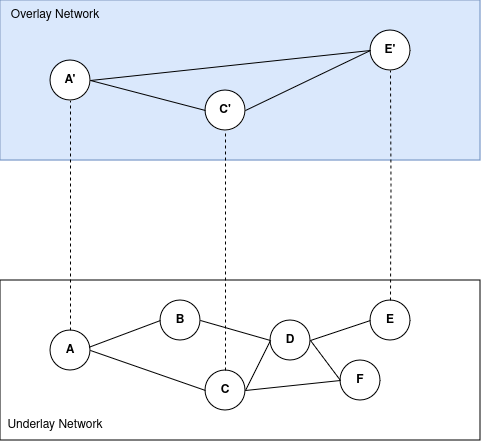
\includegraphics[width=0.5\textwidth]{overlays.png}
\caption{Concept of a very basic overlay network. Nodes A, C and E create logical links with each other, forming an overlay network}
\label{fig:overlay}
\end{figure}

\subsection{Security in Overlay Networks}

The Internet is built on public infrastructure users generally have no control over. Public routers, relay nodes, servers and even physical links always carry the risk of traffic eavesdropping and tampering by untrusted entities. Although overlay networks are able to create a logical communication structure, traffic can still be routed through this susceptible infrastructure before reaching its destination node. Therefore, to ensure the confidentiality, privacy and integrity of connections established through an insecure medium, data should be properly encrypted and authenticated.

In fact, if the Internet application running in the nodes of an overlay network has no such security considerations, communication will always be subjected to network attack vectors such as \ac{mitm} and \ac{dos} attacks and traffic snooping.

To add a confidentiality layer to communication, overlay networks employ security mechanisms which encapsulate datagrams, ensuring only designated overlay nodes can interpret the transmitted information. A common way to achieve this functionality is the use of \acp{vpn}.

\subsection{Virtual Private Networks}

Conceptually, a \ac{vpn} is a virtual network that provides functionalities  securing the transmission of data between any two endpoints ~\cite{HARMENING2017843}. \acp{vpn} have been a widely used technology for decades, establishing itself as the backbone to secure communications over the Internet.

The following sections aim to analyse how \ac{vpn} services have evolved, from its traditional design to more recent paradigms, which are able to tackle complexity and scalability issues. Then, it presents an individual overview of notable \ac{vpn} providers and compares their respective advantages, limitations, trade-offs and suitability for the scope of this solution. This state of the art technological survey aims to pickup on similar works ~\cite{zuqueteseguranca, berger2006analysis}, which examine established protocols such as OpenVPN and IPSec, while additionally reviewing modern protocols, focusing on WireGuard. This exploration serves as the foundation for understanding which protocol is the most suitable to secure communications for the scenario at hand.


\iffalse
\subsubsection{VPN Toplogies}

Not all \ac{vpn} providers have the same structural design. In fact, even individual \ac{vpn} services can be deployed to suit different use cases. Grasping the architectural capabilities and limitations of popular \ac{vpn} topologies is fundamental to evaluate the suitability of a service for a given scenario. Therefore, before individually analysing \ac{vpn} providers, this section presents a review on the advantages, disadvantages and applications of the most common \ac{vpn} topologies.

Traditional \ac{vpn} services operate under a \textbf{hub-and-spoke} architecture, a model composed by one or more \ac{vpn} Gateways - devices accepting incoming connections from client nodes and forwarding the traffic to their final destination. Hub-and-spoke architectures carry some well known bottlenecks ~\cite{ELHEDHLI20051615, o1998geographer} and, more recently, ~\cite{AN2015103}. First, it implies increased latency associated with the geographical distance between a client and the nearest hub. This topology also raises reliability issues as hubs introduce a single point of failure to the system, requiring backup plans and alternative routes to ensure no network down times.

To avoid the congestion associated with hub-and-spoke architectures, decentralized topologies have emerged which operate by establishing direct \ac{p2p} connection between clients, creating a mesh network.
\fi

\subsubsection{VPNs on NAT Networks}
\label{ss:nat-t}

A \ac{nat} is a networking mechanism responsible for translating \ac{ip} addresses in private networks to public addresses when packets sent from a private network are routed to the public Internet. In the context of \ac{vpn} communications, this process can prove to be a major constraint, not only due to \ac{nat}'s tampering of \ac{ip} packets' fields, namely destination and source addresses, which could potentially compromise its integrity in the eyes of a \ac{vpn} protocol, but also regarding the dynamically changing public \ac{ip} addresses which \ac{nat} decides to translate private addresses to. In other words, without additional tools, a host in a private network has no knowledge regarding which public \ac{ip} it will be assigned.

In fact, it is very likely that devices connected to the Internet reside in a network behind both \ac{nat} mechanisms and Firewall rules, with no open ports. Also, believing nodes will have a consistent static \ac{ip} is a very naive assumption, especially when considering mobile devices. NAT Traversal is a networking technique that enables the establishing and maintaining (by keeping \ac{nat} holes open) of \ac{p2p} connections between two peers, no matter what's standing between them, making communication possible without the need for firewall configurations or public-facing open ports. There's no one solution to achieve this functionality. In fact, there are various developments effectively implementing a NAT Traversal solution, such as ICE ~\cite{rfc8445} and STUN ~\cite{rfc8489}. Hence, each \ac{vpn} service can have its own way of supporting NAT Traversal. Each case is explored separately.


\section{VPN Providers}

\subsection{IPSec}

IPSec refers to an aggregation of layer 3 protocols that work together to create a security extension to the \ac{ip} protocol by adding packet encryption and authentication. Conceptually, IPSec presents two main dimensions: the protocol defining the transmitted packets' format, when security mechanisms are applied to them, and the protocol defining how parties in a communication negotiate encryption parameters.

Communication in an IPSec connection is managed according to \acp{sa}. A \ac{sa} is an unidirectional set of rules and parameters specifying the necessary information for secure communication to take place ~\cite{rfc4301}. Here, unidirectional means a \ac{sa} can only be associated with either inbound or outbound traffic, but never with both. Hence, an IPSec bidirectional association implies the establishment of two \acp{sa}: one for incoming packets and one for outgoing. \acp{sa} specify which security mechanism to use - either \ac{ah} or \ac{esp} - and are identified by a numeric value, the \ac{spi}. Although \ac{sa}s can be manually installed in routers, gateways or machines, it becomes impractical as more clients appear. \ac{ike} ~\cite{rfc7296} is a negotiation protocol that tackles the problems associated with manual \ac{sa} installation. In fact, \ac{ike} allows the negotiation of \ac{sa} pairs between any two machines through the use of asymmetric keys or shared secrets.

\subsubsection{Transport and Tunnel modes}

IPSec supports two distinct modes of functionality: transport and tunnel ~\cite{rfc4301}, which differ in the way traffic is dealt with and processed. In the context of \acp{vpn}, tunnel mode presents the
most desirable characteristics. First, tunnel mode encapsulates the original \ac{ip} packet, allowing the use of private \ac{ip} addresses as source or destination. Tunnel mode creates the concept of an ``outer" and ``inner`` \ac{ip} header. The former contains the addresses of the IPSec peers, while the latter contains the real source and destination addresses. Moreover, this very same encapsulation adds confidentiality to the original addresses.

Transport mode requires fewer computational resources and, consequently, carries less protocol overhead. It does not, however, provide much security compared to tunnel mode, so, to secure data in a communication, tunnel mode's total protection and confidentiality of the encapsulated \ac{ip} packet carry much more valuable functionalities.

\subsubsection{Authentication Header}

\ac{ah} is a protocol in the IPSec suite providing data origin validation and data integrity consisting in the generation of a checksum via a digest algorithm ~\cite{rfc4302}. Additionally, besides the actual message under integrity check, two other parameters are used under the \ac{ah} mechanism. First, to ensure the message was sent from a valid origin, \ac{ah} includes a secret shared key. Then, to ensure replay protection, it also includes a sequence number. This last feature is achieved with the sender incrementing a sequence integer whenever an outgoing message is processed.

\ac{ah}, as the name suggests, operates by attaching a header to the \ac{ip} packets, containing the message's \ac{spi}, its sequence number, and the \ac{icv} value. This last field is then verified by receivers, which calculate the packet's \ac{icv} on their end. The packet is only considered valid if there's a match between the sender and receiver's \ac{icv}.

Where this header is inserted depends on the mode in which IPSec is running. In transport mode, the \ac{ah} appears after the \ac{ip} header and before any next layer protocol or other IPSec headers. As for tunnel mode, the \ac{ah} is injected right after the outer \ac{ip} header.

To calculate the \ac{icv}, the \ac{ah} requires the value of the source and destination addresses, which raises an incompatibility when faced with networks operating with \ac{nat} mechanisms ~\cite{frankel2005guide}.

\subsubsection{Encapsulating Security Payload}

The \ac{esp} protocol also offers authentication, integrity and replay protection mechanisms. It differs from \ac{ah} by also providing encryption functionalities, where peers in a communication use a shared key for cryptographic operations. Analogous to the previous protocol, the \ac{esp}'s header location differs in different IPSec modes. In transport mode, the header is inserted right after the \ac{ip} header of the original packet. Also, in this mode, since the original \ac{ip} header is not encrypted, endpoint addresses are visible and might be exposed. As for tunnel mode, a new \ac{ip} header is created, followed by the \ac{esp} header.

Tunnel mode \ac{esp} is the most commonly used IPSec mode. This setup not only offers original \ac{ip} address encryption, concealing source and destination addresses, but also supports the addition of padding to packets, hampering cipher analysis techniques. Moreover, it can be made compatible with \ac{nat} and employ \ac{nat}-traversal techniques ~\cite{nam2022high, singh2012nat}.

\subsection{OpenVPN}

OpenVPN ~\cite{ovpnwebsite} is yet another open-source \ac{vpn} provider, known for its portability among the most common operating systems due to its user-space implementation. OpenVPN uses established technologies, such as \ac{ssl} and asymmetric keys for negotiation and authentication and IPSec's \ac{esp} protocol, explored in the previous section, over UDP or TCP for data encryption.

\subsubsection{TUN and TAP interfaces}

OpenVPN's virtual interfaces, which process outgoing and incoming packets, have two distinct types: TUN (short for internet TUNnel) and TAP (short for internet TAP). Both devices work quite similarly, as both simulate \ac{p2p} communications. They differ on the level of operation, as TAP operates at the Ethernet level. In short, TUN allows the instantiation of \ac{ip} tunnels, while TAP instantiates Ethernet tunnels.

\subsubsection{OpenVPN flow}

When a client sends a packet through a TUN interface, it gets redirected to a local OpenVPN server. Here, the server performs an \ac{esp} transformation and routes the \ac{ip} packet to the destination address, through the ``real" network interfaces.

Similarly, when receiving a packet, the OpenVPN server will perform decipherment and validation operations on it, and, if the \ac{ip} packet proves to be valid, it is sent to the TUN interface.

This process is analogous when dealing with TAP devices, differing, as mentioned before, at the protocol level.

\subsection{WireGuard}
\label{ss:wg}

WireGuard ~\cite{donenfeld2017wireguard} is an open-source UDP-only layer 3 network tunnel implemented as a kernel virtual network interface. WireGuard offers both a robust cryptographic suite and transparent session management, based on the fundamental principle of secure tunnels: peers in a WireGuard communication are registered as an association between a public key (analogous to the OpenSSH keys mechanism) and a tunnel source \ac{ip} address.

One of WireGuard's selling points is its simplicity. In fact, compared to similar protocols, which generally support a wide range of cryptographic suites, WireGuard settles for a singular one. Although one may consider the lack of cipher agility as a disadvantage, this approach minimizes protocol complexity and increases security robustness by avoiding vulnerabilities commonly originating from such protocol negotiation ~\cite{curguz2016vulnerabilities}.

\subsubsection{Routing}

Peers in a WireGuard communication maintain a data structure containing their own identification (both public and private keys) and interface listening port. Then, for each known peer, an entry is present containing an association between a public key and a set of allowed source \ac{ip}s.

This structure is queried both for outgoing and incoming packets. To encrypt packets to be sent, the structure is consulted, and, based on the destination address, the desired peer's public key is retrieved. As for receiving data, after decryption (with the peer's own keys), the structure is used to verify the validity of the packet's source address, which, in other words, means checking if there's a match between the source address and the allowed addresses present on the routing structure.

Optionally, WireGuard peers can configure one additional field, an internet endpoint, defining the listening address where packets should be sent. If not defined, the incoming packet's source address is used.

\subsubsection{Cipher Suite}

As mentioned before, WireGuard offers a single cipher suite for encryption and authentication mechanisms in its ecosystem. The peers' pre-shared keys are Curve25519 points, an implementation of an elliptic-curve-Diffie-Hellman function, characterized by its strong conjectured security level - presenting the same security standards as other algorithms in public key cryptography - while achieving record computational speeds ~\cite{bernstein2006curve25519}. Additionally, WireGuard's Curve25519 computation uses a verified implementation ~\cite{zinzindohoue2017hacl}, which contributes further to the robustness of the protocol's cryptography.

Regarding payload data cryptography, a WireGuard message's data is encrypted with the sender's public key and a nonce counter, using ChaCha20Poly1305, a Salsa20 variation ~\cite{bernstein2008chacha}. The ChaCha cryptographic family offers robust resistance to crypto-analytic methods ~\cite{cryptoeprint:2014/613}, without sacrificing its state-of-the-art performance.

Finally, before any encrypted message exchange actually happens, WireGuard enforces a handshake for symmetric key exchange (one for sending, and one for receiving). The messages involved in this handshake process follow a variation of the Noise ~\cite{perrin2018noise} protocol, which is essentially a state machine controlled by a set of variables maintained by each party in the process.

\subsubsection{Security}

On top of its robust cryptographic specification, WireGuard includes in its design a set of mechanisms to further enhance protocol security and integrity.

In fact, WireGuard presents itself as a silent protocol. In other words, a WireGuard peer is essentially invisible when communication is attempted by an illegitimate party. Packets coming from an unknown source are just dropped, with no leak of information to the sender.

Additionally, a cookie system is implemented in an attempt to mitigate \ac{ddos} attacks. Since, to determine the authenticity of a handshake message, a Curve25519 multiplication must be computed, a CPU intensive operation, a CPU-exhaustion attack vector could be exploited. Cookies are introduced as a response message to handshake initiation. These cookie messages are used as a peer response when under high CPU load, which is then in turn attached to the sender's following messages, allowing the requested handshake to proceed when the overloaded peer has available resources to continue.

\subsubsection{Basic WireGuard Configuration}

Connecting two peers in a WireGuard communication can be done with minimal configuration. After the generation of an asymmetric key pair and the setup of a WireGuard interface, it is only required to add the other peer to the routing table with its public key, allowed \ac{ip}s and, optionally, its internet endpoint (where it can be currently found). After both peers configure each other, the tunnel is established and packets can be transmitted through the WireGuard interface.
In a practical scenario, given two peers, \emph{A} and \emph{B}, with pre-generated keys and internet interfaces, presented on table \ref{tab:wgconfpeers}, the CLI steps to setup a minimal WireGuard communication, as specified in the official WireGuard documentation are presented in figure \ref{fig:wgconf}.


\begin{table}[]
\centering
\begin{tabular}{c|l|l|}
\cline{2-3}
\multicolumn{1}{l|}{}                            & \multicolumn{1}{c|}{\textbf{Peer A}} & \multicolumn{1}{c|}{\textbf{Peer B}} \\ \hline
\multicolumn{1}{|c|}{\textbf{Private Key}}       & gIb/+...+uF2Y=                       & aFov...G3l0=                         \\ \hline
\multicolumn{1}{|c|}{\textbf{Public Key}}        & FeQI...jHgE=                         & sg0X...7kVA=                         \\ \hline
\multicolumn{1}{|c|}{\textbf{Internet Endpoint}} & 192.168.100.4                        & 192.168.100.5                        \\ \hline
\multicolumn{1}{|c|}{\textbf{WireGuard Port}}    & 51820                                & 51820                                \\ \hline
\end{tabular}
\caption{Nodes to be configured with a WireGuard tunnel}
\label{tab:wgconfpeers}
\end{table}

\begin{figure}
\begin{multicols}{2}
\begin{lstlisting}[language=sh, frame=single, breaklines=true, breakatwhitespace=true, basicstyle=\small]
# Peer A - interface setup
$ ip link add wg0 type WireGuard
$ ip addr add 10.0.0.1/24 dev wg0
$ wg set wg0 private-key ./private
$ ip link set wg0 up

# Adding peer B to known peers
$ wg set wg0 peer sg0X...7kVA= allowed-ips 10.0.0.2/32 endpoint 192.168.100.5:51820
$

\end{lstlisting}
\columnbreak
\begin{lstlisting}[language=sh, frame=single, breaklines=true, breakatwhitespace=true, basicstyle=\small]
# Peer B - interface setup
$ ip link add wg0 type WireGuard
$ ip addr add 10.0.0.2/24 dev wg0
$ wg set wg0 private-key ./private
$ ip link set wg0 up

# Adding peer A to known peers
$ wg set wg0 peer FeQI...jHgE= allowed-ips 10.0.0.1/32 endpoint 192.168.100.4:51820
$

\end{lstlisting}
\end{multicols}
\caption{Basic WireGuard Communication Between Two Peers}
\label{fig:wgconf}
\end{figure}

\subsubsection{Limitations}
\label{sec:wglimits}

Although WireGuard proves to be a robust, performant and maintainable protocol for encrypted communication, it still presents some complexity regarding administration agility and scalability, since it (intentionally) lacks a coordination entity. New clients added to a stand-alone WireGuard network imply the manual reconfiguration of every other peer already present, a process with added complexity and prone to errors, if carried out manually.

There are, however, several software products implementing such an orchestrator, which provide functionalities to easily manage WireGuard peers and respective tunnels, such as Tailscale, Netbird or Netmaker. These solutions are explored in further sections.


\subsection{Protocol Comparison}

\subsubsection{Security}

Regarding security, although all analysed providers are capable of robustly authenticating and encrypting data, recent verifications of WireGuard's cryptographic suite \cite{lipp2019mechanised, dowling2018cryptographic} conclude WireGuard offers a smaller attack surface, when compared with OpenVPN and IPSec.

\subsubsection{Performance}

The concept of performance in \ac{vpn} applications refers to the impact the protocol has on communications. This dimension can be empirically measured, by analysing metrics like \ac{rtt}, throughput and jitter. CPU utilization is also a valuable metric, as demanding operations can also take a toll on overall network performance, since processing traffic might stall due to the CPU overloading.

The performance claims on ~\cite{donenfeld2017wireguard}, which compares WireGuard to other discussed technologies, present results in favour of WireGuard in such performance tests. This conclusion is backed by more extensive research ~\cite{mackey2020performance, osswald2020performance}, where communication is tested in a wide range of different network scenarios and CPU architectures.

WireGuard's kernel implementation and efficient multi-threading usage contribute greatly to such performance benchmarks. Overall, WireGuard outperforms IPSec and OpenVPN with no notable trade-offs.

\subsubsection{Usability}

Usability in \ac{vpn} protocols refers to the ease of use regarding service configuration and management. IPSec's configuration can be quite complex, due to its cryptographic directives and protocol negotiation. Also, the several different modes IPSec can be configured to run in might prove overwhelming for unfamiliar users. OpenVPN's GUI provides a user-friendly platform to easily administrate the software, still requiring, however, a considerable degree of technical expertise. WireGuard, however, is able to combine protocol simplicity, as it enforces a single cipher suite, with straightforward configuration directives. In fact, as we've seen in Section \ref{ss:wg}, configuring WireGuard peers requires no knowledge of the protocol's specification.

\subsection{Summary}

This section presents the fundamentals of \acp{vpn} and how they are able to ensure integrity and confidentiality to communication through insecure mediums. Then, some of the most notable \ac{vpn} providers were reviewed and compared, regarding functionalities and overall performance. The result of this analysis suggests WireGuard as the most promising \ac{vpn} protocol, due to its ease of management and configuration, security mechanisms and verified cryptography.


\section{WireGuard Coordination}
\label{sec:coordination}

In Section \ref{sec:wglimits}, the lack of a coordination entity on stand-alone WireGuard topologies was raised as a possible limitation. In fact, manually reconfiguring peers in a WireGuard network is a process that scales terribly. Moreover, on highly restrictive networks, creating direct WireGuard tunnels proves to not be as straightforward.

With such constraints in mind, this section explores applications and implementations of coordination platforms built, or with the potential to be built, on top of WireGuard, aiming to create a seamless peer orchestration and configuration process, minimizing human intervention.

\subsection{Tailscale}

Tailscale ~\cite{tailscale2020online} is a \ac{vpn} service operating with a Golang user-space WireGuard variant as its data plane. Tailscale operates under a hybrid \ac{vpn} model. Although a central entity is present, resembling hub-and-spoke architectures, its main purpose is to aid clients in configuring themselves to form a mesh network, serving nearly no traffic.

In addition to orchestrating the configuration and establishment of WireGuard tunnels, Tailscale also employs a set of mechanisms capable of addressing network constraints which would hinder the process of directly creating WireGuard connections. In fact, Tailscale praises itself as being able to make any two clients communicate, regardless of the network structure and security policies standing in-between them. For the scope of this project, where very few is known about \ac{ua}'s network, the ability to bypass such constraints would prove extremely valuable.

This section explores how Tailscale is able to manage the WireGuard links between its clients, creating a WireGuard encrypted overlay network while dealing with security constraints preventing such communications to take place.

\subsubsection{Architecture}

Tailscale's central entity, referred to as the \textbf{coordination server}, functions as a shared repository of peer information, used by clients to retrieve data regarding other nodes and establish on-demand WireGuard connections among each other.

This approach differs from traditional hub-and-spoke since the coordination server carries nearly no traffic, it only serves encryption keys and peer information. Tailscale's architecture provides the best of both worlds, benefiting from the advantages of a centralized entity facilitating dynamic reconfigurations and peer discovery without bottlenecking WireGuard's data exchanging performance.

In practical terms, a Tailscale client will store, in the coordination server, its own public key and where it can currently be found. Then, it downloads a list of public keys and addresses that have been stored on the server previously by other clients. With this information, the client node is able to configure its Tailscale interface and start communicating with any other node in its domain.

\subsubsection{Overcoming restrictive networks}
\label{ssec:tsnetworks}

There are, however, some network security configurations which prevent WireGuard tunnels from being established. For example, firewalls blocking \ac{udp} traffic entirely prevent the creation of direct WireGuard tunnels between two peers. In addition to orchestrating WireGuard peers, Tailscale is also able to overcome such constrained networks.

Regarding stateful firewalls, where, generally, inbound traffic for a given source address on a non-open port is only accepted if the firewall has recently seen an outgoing packet with such \emph{ip:port} as destination, Tailscale keeps, in its coordination server, the public address of each node in its network. With this information, if both peers send an outgoing packet to each other at approximately the same time (a time delta inferior to the firewall's cache expiration), then the firewalls at each end will be expecting the reception of packets from the opposite peer. Hence, packets can flow bidirectionally and a \ac{p2p} communication is established. To ensure this synchronism of attempting communication at approximate times, Tailscale uses its coordination server and \ac{DERP} servers (explored further in the following paragraphs) as a side channel.

Although this procedure is quite effective, in networks with \ac{nat} mechanisms, where source and destination addresses are tampered with, this process is not as straightforward, since peers don't know the public addresses \ac{nat} will translate their private addresses to. The \ac{stun} protocol offers aid in performing \ac{nat}-traversal operations ~\cite{rfc8489} and can solve this problem. For a peer to discover and store in the coordination server its own public \emph{ip:port}, it first sends an \ac{udp} \ac{ip} binding request to a \ac{stun} server. Upon receiving this packet, the \ac{stun} server can see which public source address was used (the address \ac{nat} translated to) and replies this value to the peer.

There are, however, some \ac{nat} devices that create a completely different public address mapping for each different destination a machine communicates with, which hinders the above address discovery process. Such devices are classified as \ac{edm} (in opposition to \ac{eim}) ~\cite{rfc4787}.

Networks employing \ac{edm} \ac{nat} devices and/or really strict firewall rules, render these traversal techniques useless. To enable \ac{p2p} communications in such scenarios, Tailscale also provides a network of \ac{DERP} servers, which are responsible for relaying packets over \ac{http}. A Tailscale client is able to forward its encrypted packets to one of such \ac{DERP} servers. Since a client's private key never actually leaves its node, \ac{DERP} servers can't decrypt the traffic being relayed, performing only redirection of already encrypted data. Tailscale offers a geographically distributed fleet of such servers. However, since traffic is encapsulated as an \ac{http} stram, relayed communications always imply a degradation of network performance, which isn't terrible, as the alternative is not being able to communicate at all.

Hence, Tailscale connections can be of two types: either \textbf{direct} or \textbf{relayed}. Tailscale will always attempt to create direct connections. In fact, if \ac{nat}-traversal succeeds on both endpoints and there are no restrictions to \ac{udp} traffic, a direct WireGuard tunnel can be established. However, on networks employing \ac{edm} \ac{nat} mappings and/or \ac{udp} blocking firewalls, direct connections cannot be formed. That's where relayed connections are created. Clients on relayed connections encapsulate WireGuard \ac{udp} packets as \ac{tcp} streams and forwards them through \ac{http} to the closest \ac{DERP} server available, which in turn delivers them to its destination.

\subsubsection{Headscale}
\label{sec:hs}

While Tailscale's client is open source, its coordination server isn't. There is, however, an open-source, self-hosted alternative to Tailscale's control server, Headscale. Headscale ~\cite{headscale2023online} provides a narrow-scope implementation (with a single Tailscale private network) of the aforementioned control server, which, in the authors' words, is mostly suitable for personal use and small organizations. Nodes running Tailscale clients can opt to specify the location of the control server, which can be the address of a running self-hosted Headscale instance.

Headscale also supports the self-hosting of \ac{DERP} and \ac{stun} servers. This is useful as it allows the self-hosting of a complete Tailscale solution.

\section{University of Aveiro Network}
\label{sec:uanet}

Due to security and privacy concerns, the specification of the \ac{ua}'s network topology is not publicly available nor is it made available for this dissertation. As such, it is perceived as a black box. There are, however, a few reachable conclusions derived from observing its behaviour.

First, that the network is highly segmented, where clients are grouped according to their roles. In fact, when clients connect to an \ac{ap} within the campus, they are connected to a \ac{vlan} shared by several other clients, in which the private resources are accessible. Regarding \ac{nat}, the present mechanisms in the network are unknown, as are their mappings' \ac{ttl}, which is an important variable mentioned in Section \ref{ssec:tsnetworks} to perform \ac{nat}-traversal techniques.

Any other specification of \ac{ua}'s network is unknown.

\section{Robot Operating System}

TODO


\chapter{Methodology}
\label{chapter:method}

Having outlined the relevant research, background and technologies for this dissertation's context, this chapter aims to present a work proposal for the solution implementation. The approach to be taken is segmented in three main stages: Prototype Development, Production Deployment and, finally, Automation.

\section{Technology Stack}

Based on the research done in the previous section, WireGuard seems the most adequate encrypted communication protocol for this project. However, to avoid the already covered added complexity of managing a stand-alone WireGuard network, Tailscale will function as the core of this solution. Ideally, all Tailscale related infrastructure should be self-hosted, which can be achieved using Headscale's open-source implementation of Tailscale's coordination server.

Therefore, our overlay networks are formed by a group of Tailscale clients, running in the robots, which are managed and coordinated by a self-hosted Headscale coordination server.

\section{Prototype Development}
\label{sec:protodev}

This first phase aims to build a small-scale prototype in a development environment. The prototype should, using Headscale as the coordination server and Tailscale as clients, be able to establish a \ac{p2p} connection between two sample machines, which couldn't communicate beforehand. Hence, this phase's main goals are to (i) create a virtual environment which simulates the scenario being tackled, (ii) establish \ac{p2p} connections between clients behind private \ac{nat} networks  and (iii) validate the communication through the \ac{ros} middleware. Obviously, regarding goal (i), the simulation of the networking conditions can't be entirely accurate, since, as referenced in section \ref{sec:uanet}, details regarding \ac{ua}'s network mechanisms are vastly unknown. It is possible, however, to create an analogous situation, where clients can't immediately form \ac{p2p} communications with each other but can all communicate with an external, public server. Moreover, as stated in previous sections, Tailscale's protocol efficiently deals with most network constraints preventing direct communication. In other words, it is only known clients can't communicate, the reasons behind why they can't are abstracted by Tailscale.

This environment must be composed of three entities: a public server and two clients in their own isolated networks. As mentioned in section \ref{sec:hs}, Headscale is an open-source implementation of Tailscale's control server. Thus, the control server in this environment shall be a self-hosted Headscale instance deployed in the public server. Both clients, which can reach the public server, but not each other, should then authenticate in this control server and configure their Tailscale interfaces and addresses, allowing for a direct communication to take place.

In order to validate goal (iii), a simple \ac{ros} application should be deployed and tested in the clients, in which communication is done through the Tailscale interfaces.

\section{Deployment}

After achieving and configuring the prototype previously developed, the next phase focuses on the deployment of the solution within \ac{ua}'s premises. As already mentioned, the Headscale instance should be hosted in a server accessible from anywhere within the campus. Here, the configuration should be based on the research done during the previous phase, with few eventual changes to ports and/or addresses. Regarding clients, ideally, each team of robots should have its own user, which individual robots will use for authentication. <TODO: COMO SERA O PROCESSO DE GERAR KEYS???>.

Hence, this phase aims to (i) deploy an Headscale server available to any client connected to \ac{ua}'s network, (ii) configure robots to act as Tailscale clients and (iii) establish secure communication between a team of robots spread throughout the campus.


\section{Validation}
\label{sec:metvalidation}

Validating the solution requires an analysis of Tailscale's overhead on  network performance, which should ensure suitable results to use in \ac{ros} applications. This includes collecting metrics like \ac{rtt}, throughput, jitter and packet loss both on regular and Tailscale connections. Also, clients should be able to join the overlay networks from anywhere in the campus. So, the goals for these experiments are to (i) measure network performance on regular vs Tailscale connections, (ii) validate connections spread out through various campus points and (iii) test the solution with demanding apps, such as live video streaming, through Tailscale interfaces.

\section{Automation}
\label{sec:automethod}

This final development phase aims to create automation processes to aid in the deployment and configuration of the solution.

So, the automation process has two main goals in mind: First, to (i) provide a minimal configuration script to install and deploy an Headscale instance and provision its respective resources (auth keys, users, \acp{acl}) and (ii) provide a script installing Tailscale's client and configuring the system to be ready to join a desired network.

\section{Work Plan}

The tasks encompassing the phases described above can be summed up in a Gantt diagram, presented in figure \ref{fig:gantt}. The tasks to be carried out are as follows:

\begin{itemize}
  \item \textbf{Prototype Development} - Implementation, in the development environment, of a prototype fulfilling the requirements. The end goal is to establish a \ac{p2p} connection between the two machines that can't communicate.
  \item \textbf{Deployment} - Deployment of the control server in \ac{ua}'s public services domain and configuration of clients in the robots.
  \item \textbf{Validation} - Validation of the deployed solution, ensuring encrypted communication between nodes in different geographical locations within the campus.
  \item \textbf{Automation} - Development of configuration based scripts automating client and server deployment and configuration.
  \item \textbf{Final Document Writing} - Writing of the final document, presenting the development process and providing analysis of respective results.
\end{itemize}

\begin{figure}[h]
\centering
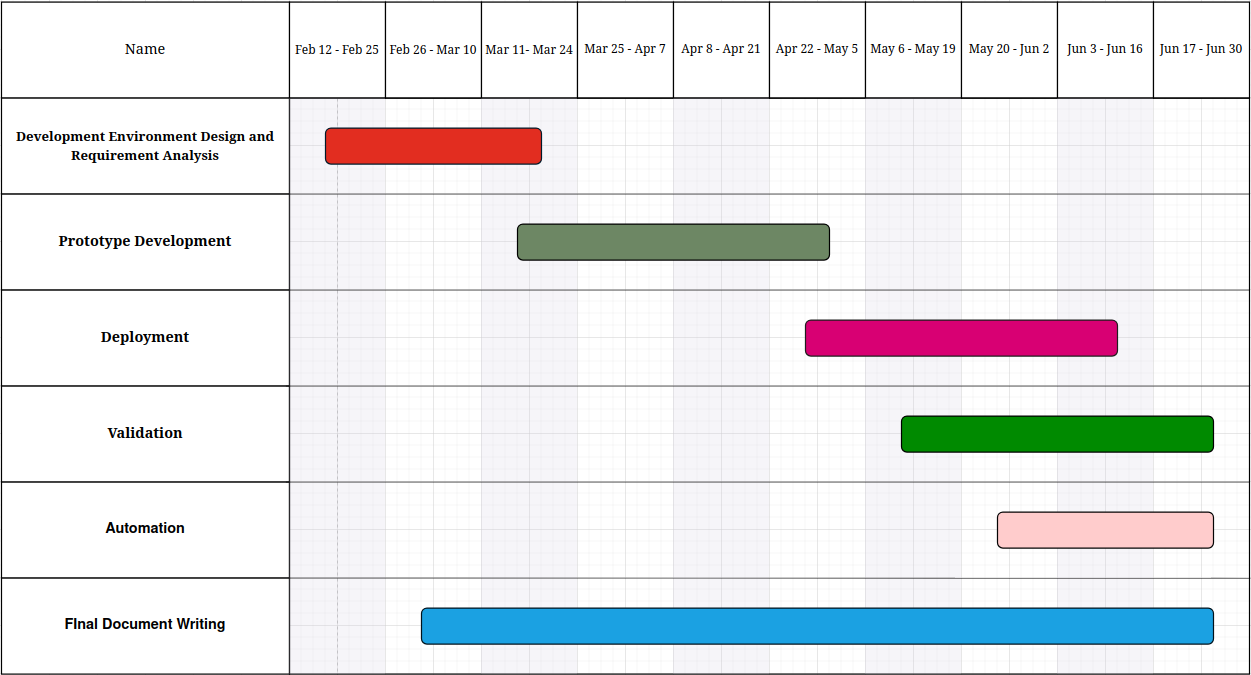
\includegraphics[width=1\textwidth]{gantt.png}
\caption{Development planning proposal}
\label{fig:gantt}
\end{figure}


\chapter{Architecture}

This chapter details the architectural specification of our solution. In the previous section, Tailscale was explored as a WireGuard orchestrator, capable of establishing \ac{p2p} tunnels regardless of the security mechanisms present in the network. It was also noted that, although Tailscale's client is open source, its coordination server isn't. As this solution is meant to be entirely deployed within the university's premises, we are required to self-host Tailscale's central entity and related infrastructure, namely \ac{stun} and \ac{DERP} servers. Finally, these services must be made available to any client even before joining the overlays, as the coordination server handles operations such as authentication and address advertisement.

To self-host a Tailscale coordination server, Headscale, explored in section \ref{sec:hs}, will function as the solution's central entity. In addition to providing a Tailscale orchestrator alternative, Headscale allows the configuration and deployment of an embedded \ac{DERP} server, which also exposes \ac{stun} endpoints. As such, all necessary central services are configured and managed via Headscale.

Clients will run the open-source Tailscale's node software, a package composed by a \ac{cli} and a daemon. Tailscale's daemon is the entity responsible for communicating with the orchestrator, while the \ac{cli} offers an interface to control and execute operations through the daemon.

Figure \ref{fig:arch} depicts the solution's architecture.

\begin{figure}[h]
\centering
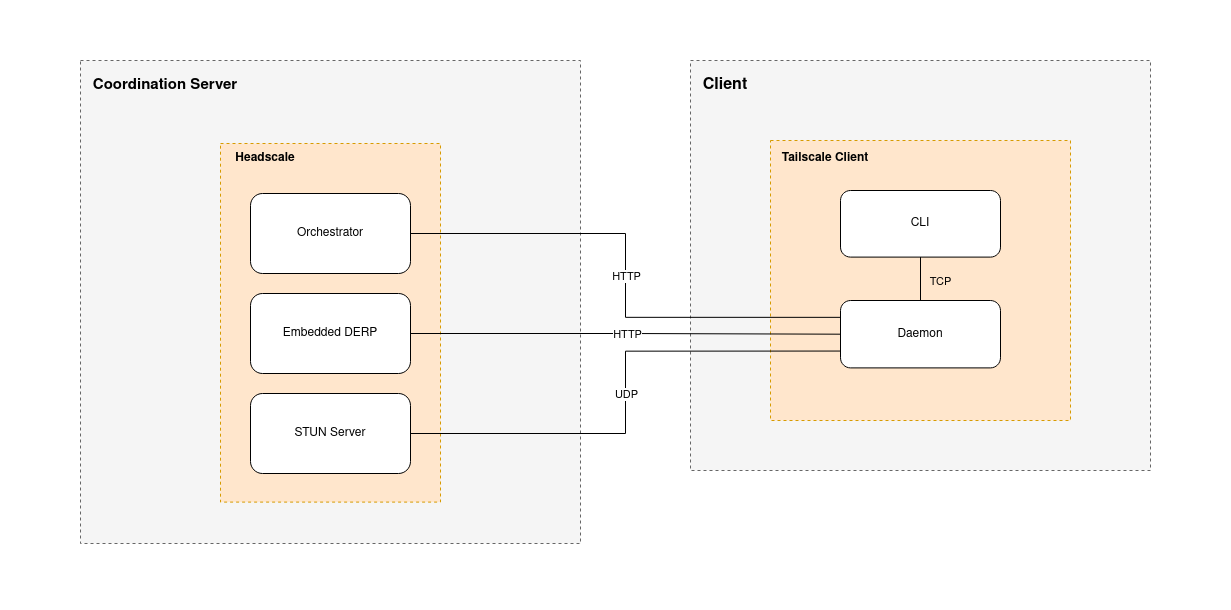
\includegraphics[width=1\textwidth]{arch.png}
\caption{Solution's Architecture}
\label{fig:arch}
\end{figure}

\section{Coordination Server}

The coordination server is the central entity responsible for offering clients functionalities to configure themselves and aid in establishing communications when dealing with highly restrictive networks. It is composed of three main services, an orchestrator, a packet relaying service and an endpoint to perform \ac{nat}-traversal. This section explores the operations of each of these components and their respective roles in the protocol.

\subsection{Orchestrator}

The orchestrator implements most configuration and coordination operations.

\subsection{Relay Server (DERP)}

In Section \ref{ssec:tsnetworks}, two types of Tailscale connections were presented, direct and relayed. While the Tailscale protocol always attempts to establish direct connections first, on highly constrained networks, where \ac{nat}-traversal is unsuccessful or \ac{udp} traffic is entirely forbidden, Tailscale encapsulates encrypted WireGuard packets as \ac{tcp} and transmits them to a relay server, refered to as a \ac{DERP} server, over \ac{http}. In other words, an overlay node communicating through one of such networks is able to perform this encapsulation process and forward packets to a relay. The relay server is then responsible for delivering the message to its destination. Hence, for relayed communications to be established, the orchestrator must advertise which \ac{DERP} servers are available for clients to transmit packets to.

While Tailscale's official coordination server offers a fleet of geographically distributed \ac{DERP} servers, the coordination server in this solution is also a self-hosted instance, as our scope is to exclusively serve \ac{ua}'s clients. Fortunately, Headscale supports the deployment of an embedded \ac{DERP} server, which runs alongside the orchestrator's main service.

\subsection{NAT-Traversal Server (STUN)?}

Finally, the coordination server is also required to expose an endpoint for clients to discover which public \ac{ip} they should advertise to the orchestrator and to perform \ac{nat}-traversal, a fundamental operation explored in Section \ref{ss:nat-t}. Headscale performs \ac{nat}-traversal using the \ac{stun} protocol.

Clients will perform \ac{ip} binding requests to a \ac{stun} server through \ac{udp} messages and receives its public \ac{ip} and port (generated by \ac{nat}) as a response.

\section{Client}

\subsection{Command Line Interface}

\subsection{Daemon}


\chapter{Implementation}

\chapter{Experiments and Results}
\label{chap:results}

In order to validate the developed solution, several experiments were conducted which provide us with insights regarding the overlay networks' communication performance, security and usability in the context of \ac{ros} applications. Hence, this chapter details the procedures taken for results and metrics gathering, followed by their respective analysis and derived conclusions.

\section{Network Performance}

Network performance is understood as the quality of the communication in the eyes of an overlay node. Measuring network performance requires the collection  and visualization of metrics produced while data is being exchanged on the overlay networks. For the scope of our conclusions, four of such metrics were gathered, on connections happening in distinct scenarios.

The metrics we chose for this experiment provide insights on three distinct dimensions, outlined in ~\cite{livronet, Hanemann2006}.

\subsubsection{Delay}

Delay in network performance refers to the time packets take to be transmitted from a source to a destination, through its communication medium. Network congestion, insufficient computational resources and routing rules can directly influence this dimension. To measure the delay associated with a connection, two metrics are considered, Round Trip Time (\ac{rtt}) and jitter.

\ac{rtt} times dictate how long a source has to wait to receive a response from its destination, while jitter measures the variation of packet arrival times. High jitter has an impact on the smoothness of a connection, generally having noticeable negative effects on real time communications and media streaming \cite{claypool1999effects}.

\subsubsection{Bandwidth and Throughput}

Bandwidth is a dimension perceived as the maximum amount of information capable of being transmitted through a connection in a given time interval. Throughput, while also measuring the amount of transmitted data over time, assess how much data in a given communication is actually transferred by unit of time. In other words, measuring throughput allows us to understand the rate at which data is transmitted between a source and a destination, while bandwidth measures the network's total capacity. Network throughput can be calculated by executing demanding packet transmissions between any two nodes and measuring how much information is transmitted on a given time delta.

\subsubsection{Losses and Errors}

Finally, this dimension tackles how much information is not correctly transmitted and is measured by calculating a communication's packet loss, the fraction of packets sent which don't arrive at a destination. Losing packets implies traffic retransmissions, which contribute negatively to the overall network performance.

\subsection{Metric Gathering}
\label{ss:metrics}

The metrics to be gathered for network performance analysis are \textbf{\ac{rtt}} and \textbf{jitter} regarding delays, \textbf{throughput} and maximum \textbf{bandwidth} for information transfer rate and \textbf{packet loss} to assess any issues regarding packets not being properly transmitted.

There are numerous open source tools which measure most of these metrics by running configurable network tests. One such example is iperf ~\cite{iperfws}. Iperf operates by exchanging packets through a client-server model and offers tests capable of collecting both \ac{tcp} and \ac{udp} throughput and bandwidth, network jitter and packet loss. \ac{rtt} times are calculated by exchanging a given number of \ac{icmp} packets and measuring communication travel times, achievable with simple \textbf{ping} commands.

These processes were automated using a python script \footnote{https://github.com/VascoRegal/ua-overlays-automation/blob/main/tests/network/iperf/run.py}. This script starts by connecting to an iperf server and running \ac{tcp} and \ac{udp} iperf tests, outputting its results as \ac{json}. Then, to the same host running the iperf server, \ac{icmp} packets are exchanged, calculating \ac{rtt} minimum, maximum, mean and deviation values, which are also appended to the previously produced \ac{json} object. These results are finally exported to a file for later processing. The duration of each iperf test and the total number of \ac{icmp} packets exchanged for \ac{rtt} calculations are both configurable variables.

The result files produced by running this script allows us to build a dataset containing the necessary metrics, used to draw the conclusions present further in this chapter.

\subsection{Running Experiments}

Having defined the relevant metrics to evaluate communication performance through the overlays and development of a script which automates the results gathering processes, experiments are ready to be run between any two overlay nodes. Since communication is possible through Tailscale relayed connections regardless of clients' physical locations, we can collect insights from multiple campus points. This will not only allow us to understand the performance of the solution and how it behaves with geographical distance but also ensure the overlays can be used from anywhere within \ac{ua}'s premises.

For these experiments, an overlay node running an iperf server was deployed in \ac{iris}, connected to \ac{ua}'s network. Then, with another machine, the experiment script was run, pointing the iperf server as the \ac{iris}'s node's Tailscale \ac{ip}, from disperse campus' locations. Table \ref{tab:locs} presents the selected test case buildings.

Regarding test configuration, both \ac{tcp} and \ac{udp} iperf tests were run for 10 minutes each. Regarding \ac{rtt} calculations, a total of 100 \ac{icmp} replies were used.

\subsection{Analysis and Conclusions}


TODO

\iffalse
\section{Protocol Overhead}

To validate the solution's performance, two dimensions must be taken into account. First, it is necessary to ensure clients can use the overlay networks from anywhere within the campus. Then, the overall network performance must also be analysed, namely communication latencies, network \ac{tcp} throughput, \ac{udp} packet loss and maximum bandwidth and network jitter. Fortunately, both scopes can be tested simultaneously! \textbf{iperf3} is an open-source tool which collects such metrics by exchanging packets on a client-server model.

Therefore, these tests were implemented as a python script \footnote{https://github.com/VascoRegal/ua-overlays-automation/blob/main/tests/network/iperf/analysis.py} which connects to a host to run \textbf{iperf3} \ac{tcp} and \ac{udp} tests for 120 seconds each and exporting the results as \ac{json}. \textbf{iperf3}'s \ac{tcp} tests collect \ac{tcp} network throughput and minimum, maximum and mean \ac{rtt} time. \ac{udp} tests collect network jitter and packet loss.

For this experiment, a Tailscale client running \textbf{iperf3} as a server was placed inside \ac{iris}'s network. Then, with another machine, the script was run in clients connected to \ac{ua}'s network, from disperse points in the campus. This procedure allows not only the collection of \textbf{iperf3}'s network metrics and latencies but also the validation of the solution's coverage, since the script connects to the \ac{iris}'s host with its Tailscale \ac{ip}. If this connection fails, Tailscale can't cover that area, possibly due to more constraining networking rules. As it will be shown in the following section, however, none of the tested areas failed to establish communication.

Twelve different test scenarios were run under similar conditions, presented on table \ref{tab:locs}. Since the \textbf{iperf3} server is running on \ac{iris} network, tests can be executed either using the server's Wi-Fi interface or its Tailscale interface. Interpolation of the data from these two scenarios allows the visualization of Tailscale's overhead on communication. The remaining cases are meant to both ensure Tailscale can establish connections from any point in the campus, while also providing insights on overall network performance.
\fi

\begin{table}[]
  \centering
\begin{tabular}{|c|c|c|}
\hline
\textbf{Location}                                                                                             & \textbf{\begin{tabular}[c]{@{}c@{}}Building\\ ID\end{tabular}} & \textbf{\begin{tabular}[c]{@{}c@{}}Connection\\ Type\end{tabular}}     \\ \hline
\begin{tabular}[c]{@{}c@{}}University Library\\ (BIB)\end{tabular}                                          & 17                                                                 & \begin{tabular}[c]{@{}c@{}}Tailscale\\ (relayed)\end{tabular} \\ \hline
\begin{tabular}[c]{@{}c@{}}Political Science Department\\ (DSCPT)\end{tabular}                              & 12                                                                 & \begin{tabular}[c]{@{}c@{}}Tailscale\\ (relayed)\end{tabular} \\ \hline
\begin{tabular}[c]{@{}c@{}}Communication and Arts Department\\ (DECA)\end{tabular}                          & 21                                                                 & \begin{tabular}[c]{@{}c@{}}Tailscale\\ (relayed)\end{tabular} \\ \hline
\begin{tabular}[c]{@{}c@{}}Student's Bar\\ (BE)\end{tabular}                                                  & N                                                                  & \begin{tabular}[c]{@{}c@{}}Tailscale\\ (relayed)\end{tabular} \\ \hline
\begin{tabular}[c]{@{}c@{}}Eletronics, Telecomunications and Informatics\\ Department\\ (DETI)\end{tabular} & 4                                                                  & \begin{tabular}[c]{@{}c@{}}Tailscale\\ (relayed)\end{tabular} \\ \hline
\begin{tabular}[c]{@{}c@{}}Exhibition Hall\\ (EXPO)\end{tabular}                                              & 24                                                                 & \begin{tabular}[c]{@{}c@{}}Tailscale\\ (relayed)\end{tabular} \\ \hline
\begin{tabular}[c]{@{}c@{}}Pedagogical Complex\\ (CP)\end{tabular}                                            & 23                                                                 & \begin{tabular}[c]{@{}c@{}}Tailscale\\ (relayed)\end{tabular} \\ \hline
\begin{tabular}[c]{@{}c@{}}Mathematics Department\\ (DMAT)\end{tabular}                                     & 11                                                                 & \begin{tabular}[c]{@{}c@{}}Tailscale\\ (relayed)\end{tabular} \\ \hline
\begin{tabular}[c]{@{}c@{}}Biology Department\\ (DBIO)\end{tabular}                                         & 8                                                                  & \begin{tabular}[c]{@{}c@{}}Tailscale\\ (relayed)\end{tabular} \\ \hline
\begin{tabular}[c]{@{}c@{}}Economics and Management Department\\ (DEGEIT)\end{tabular}                      & 10                                                                 & \begin{tabular}[c]{@{}c@{}}Tailscale\\ (relayed)\end{tabular} \\ \hline
\end{tabular}
\caption{Locations used for network performance analysis}
\label{tab:locs}
\end{table}

\section{Protocol Overhead}

Cmmunicating with the Tailscale protocol implies additional operations  to take place on sending and receiving data, which introduces an overhead to the general network performance. In fact, data encryption, security mechanisms and transmission of additional Tailscale protocol packets produce a toll on the regular network behaviour. Moreover, as connections within the university's network are relayed, meaning traffic is being redirected over \ac{http}, also contributes to the degradation of network performance. To understand this dimension, this section presents an experiment which provides insights on said protocol overhead, regarding network delay and throughput.

This experiment aims to measure Tailscale's overhead on communication, by interpolating data collected, under very similar conditions, from a connection through a regular Wi-Fi interface against a connection done through Tailscale tunnel.

Such a scenario can be achieved with two clients residing inside \ac{iris}. With both machines connected to \ac{iris}'s private network, they can communicate directly via private \acp{ip}, hence metrics were collected with the script described in Section \ref{ss:metrics}. Then, the same metric gathering was run for the same scenario, with one of the clients connected to \ac{ua}'s network and the test done via Tailscale \acp{ip}.

\subsection{Results and Analysis}

The two generated datasets allow us to visualize how Tailscale impacts network performance. Figure \ref{fig:overhead} presents the \ac{tcp} throughputs for the both experiments, while figure \ref{fig:latency_overhead} compares the \ac{rtt} distributions. Analysing the figures corroborates the idea that communicating through relayed Tailscale connections implies a considerable loss in network performance. To be able to represent this performance depletion numerically, we can calculate the relative change between the two measurements, using the percent log-change formula \cite{tornqvist1985should}.

The percent log-change is a numerical indicator of the change between two groups of values. In the context of this analysis, the percent log-change represents how much throughput was lost and how \ac{rtt} times increased, when comparing the internal and tunnel connections. We chose to use the log-change as an indicator instead of directly calculating the percentage change as it outputs a symmetric indicator, abstracting the necessity of choosing one connection as the baseline. The percent log-change is given by the expression:

\[
\text{Log-Change (\%)} = \ln\left(\frac{y}{x}\right) \times 100
\]

Where \textbf{y} and \textbf{x} are the two set of values under comparison. Using the average measurements generated by the network tests, throughput loss can be calculated with the expression:

\[
\text{Throughput Loss (\%)} = \ln\left(\frac{\overline{\text{TP}}_I}{\overline{\text{TP}}_T}\right) \times 100
\]

Where \textbf{ \( \overline{\text{TP}}_I \)} is the average throughput for the internal connection and \textbf{\( \overline{\text{TP}}_T \)} is the average throughput for the Tailscale connection, which results in a throughput loss of \textbf{46.23} \%

The same procedure can be applied to the measured \ac{rtt} values:

\[
\text{RTT Increase (\%)} = \ln\left(\frac{\overline{\text{RTT}}_I}{\overline{\text{RTT}}_T}\right) \times 100
\]

Similarly, \textbf{ \( \overline{\text{RTT}}_I \)} is the average \ac{rtt} times for the internal connection while \textbf{\( \overline{\text{RTT}}_T \)} is the average \ac{rtt} times for the Tailscale connection. This calculation results in an \ac{rtt} increase of \textbf{21.11} \%

These two indicators give us a perception of Tailscale's overhead. TODO: Concluir melhor

\begin{figure}[h]
\centering
  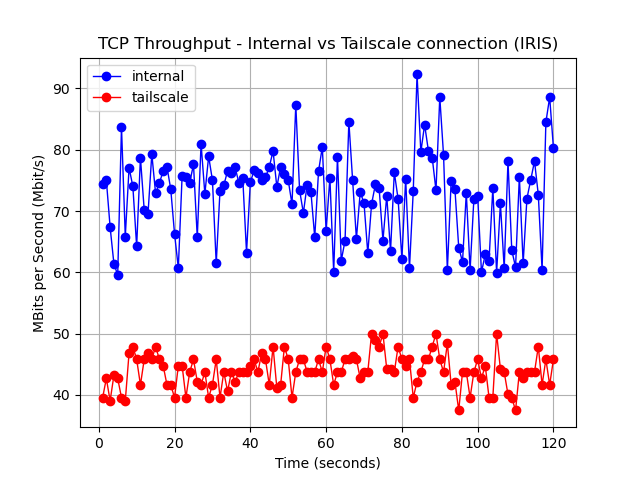
\includegraphics[width=0.9\textwidth]{overhead.png}
  \caption{Tailscale's toll on throughput, tested on internal and Tailscale connections inside IRIS-Lab}
  \label{fig:overhead}
\end{figure}

\begin{figure}[h]
\centering
  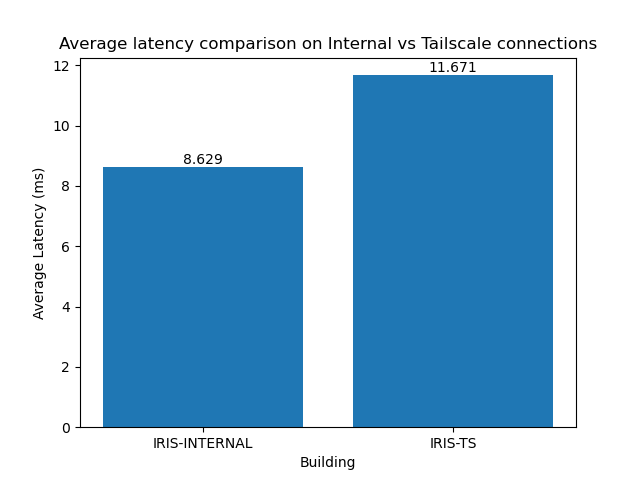
\includegraphics[width=0.8\textwidth]{latency_overhead.png}
  \caption{Round Trip Time distribution for internal (IRIS-I) and Tailscale (IRIS-TS) connections}
  \label{fig:latency_overhead}
\end{figure}

\begin{figure}[h]
\centering
  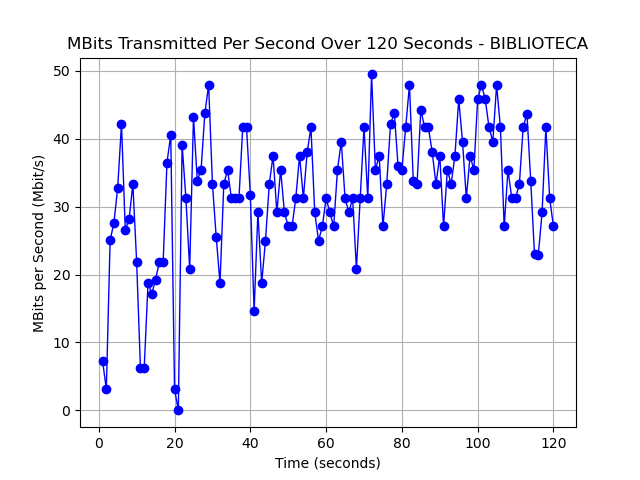
\includegraphics[width=0.8\textwidth]{biblioteca-tcp.png}
  \caption{TCP Tailscale tunnel Network TCP Throughput (University Library)}
  \label{fig:tcptplibrary}
\end{figure}


\begin{figure}[h]
\centering
  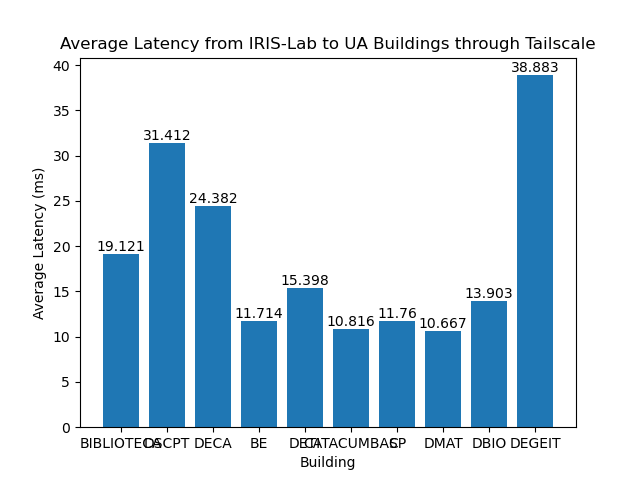
\includegraphics[width=0.8\textwidth]{building-latency.png}
  \caption{Average RTT times by campus location}
  \label{fig:buildlat}
\end{figure}


\begin{figure}[h]
\centering
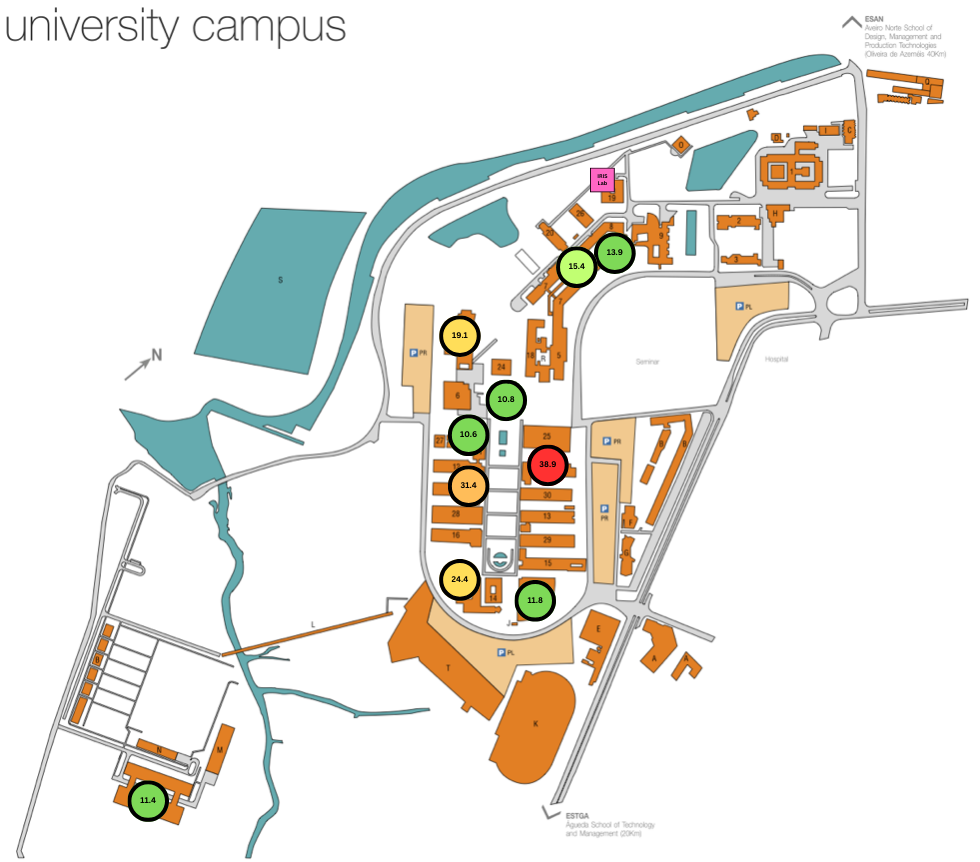
\includegraphics[width=0.8\textwidth]{ua-latency.png}
\caption{Average RTT on a Tailscale connection from different UA buildings to IRIS-Lab. The numbers in the circles represent average RTT values, in ms.}
\label{fig:ualats}
\end{figure}


\begin{figure}[h]
\centering
  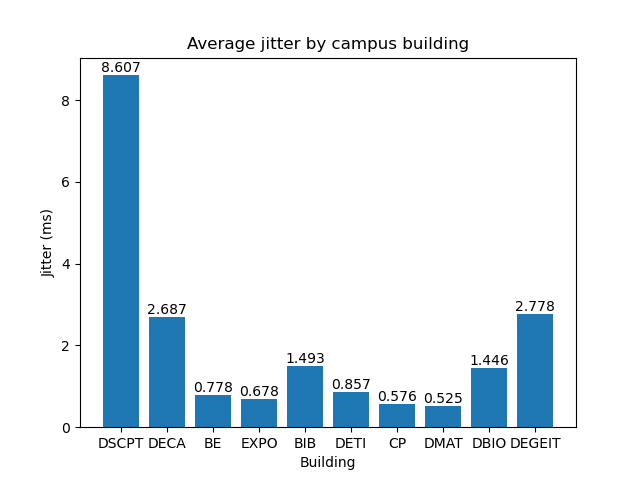
\includegraphics[width=0.8\textwidth]{building-jitter.png}
  \caption{Network Jitter by campus location.}
  \label{fig:uajitter}
\end{figure}


\section{Security and Confidentiality}

As we have seen, Tailscale encrypts and secures communications with WireGuard. This experiment aims to visualize how packets in the overlays are perceived by untrusted entities. A straightforward method to verify this dimension relies on the analysis of network captures. In fact, messages in a Tailscale tunnel can only be understood by the source and destination nodes. Traffic travelling through any other infrastructure is seen as an undecipherable stream of packets.

Hence, this validation operates by generating traffic between two overlay nodes and simultaneously capturing the packets in the destination node's Tailscale interface and in another intermediary network link's interface. On relayed connections, which is the case in this scenario, this intermediary capture is done in the \ac{DERP} server's interface. We can verify the encryption taking place by correlating packets from both captures using their timestamps as reference.

\subsection{Capturing and Visualising Traffic}

To capture packets on a network interface, \textbf{Tcpdump} \cite{tcpdump}, an open source command-line tool, was used. With this tool, we can initiate a capture by using the \textbf{tcpdump} command and pointing to a desired interface. Results from a capture can be exported to a file, which then allows a user friendly visualisation using \textbf{Wireshark} \cite{wireshark}, also an open source tool. Wireshark facilitates analysing and correlating the captures.

\subsection{Generating Traffic}

For the scope of this experiment, a client server scenario was created using two overlay nodes. One of the nodes runs a simple \ac{http} server, listening on its Tailscale interface, while the other generates traffic by executing requests to this server using \textbf{curl} \cite{curl}. Both nodes are connected to \ac{ua}'s network, hence the Tailscale connection is relayed.

\subsection{Running the experiment}

Having defined how traffic is generated and captured, the experiment starts by initiating two captures, one on the \ac{http} server's Tailscale interface and one on the \ac{DERP} server's Wi-Fi interface. Traffic associated with the generated \ac{http} requests will travel through both these interfaces, as all Tailscale traffic requires relaying by the \ac{DERP} server before reaching its respective destination.

With the captures running, \ac{http} requests were done by the client node, using cURL. After closing the captures, two pcap files are generated, which are loaded in Wireshark and correlated manually by analysing the packets' timestamps.

\subsection{Results}

Figure \ref{fig:cipher} presents both captures side by side in Wireshark. By analysing these results, the \ac{http} request and response are encapsulated as a \ac{tcp} stream on the \ac{DERP} capture, and its payload encrypted, while the corresponding packets in the \ac{http} server's interface capture shows the same request and response as plain-text. Hence, Tailscale is effectively encrypting tunnel traffic, as only communication end nodes are able to decrypt and understand the information being transmitted.

\begin{figure}[h]
\centering
  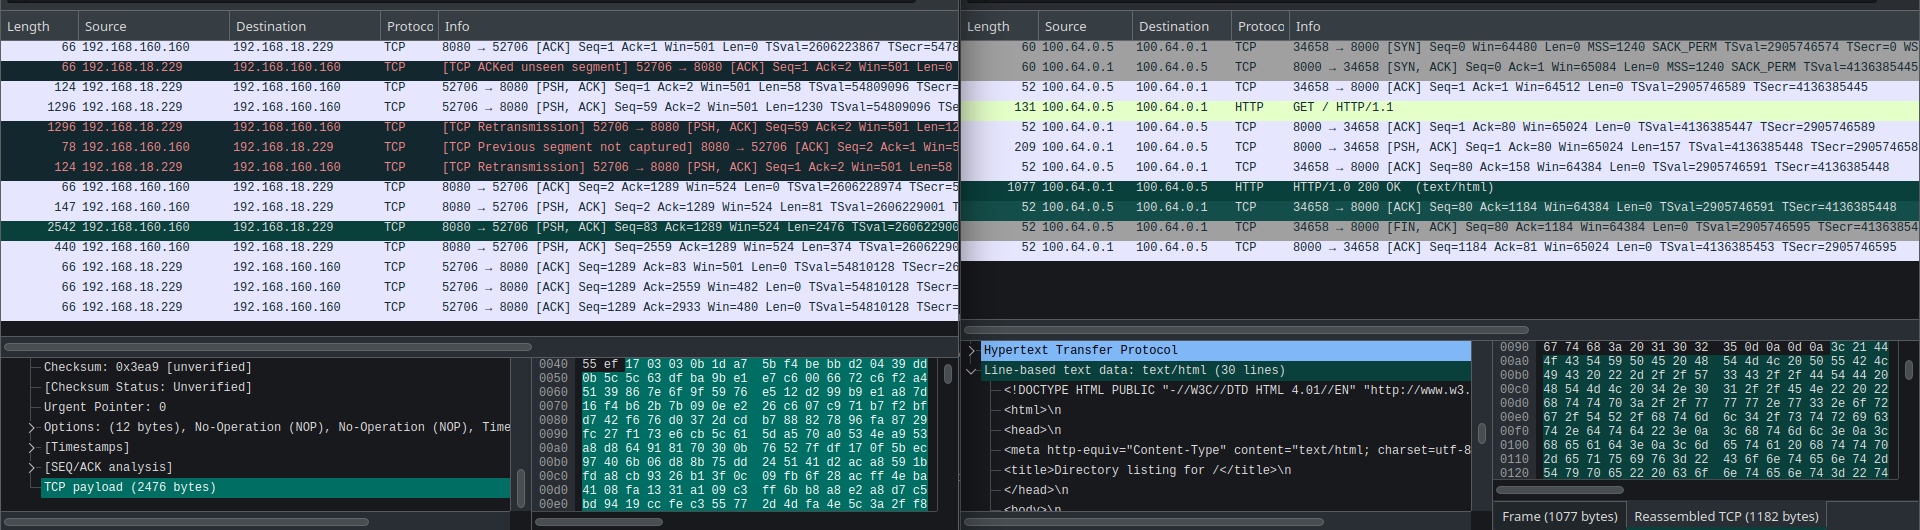
\includegraphics[width=0.9\textwidth]{cipher.png}
  \caption{TCP Streams from external capture (left) and destination node capture (right)}
  \label{fig:cipher}
\end{figure}

\section{Chapter Summary}

This chapter presented how this solution was validated and its performance analysed. To collect network performance metrics, \textbf{iperf3} was used in a range of different scenarios. First, to gain insights on Tailscale's overhead, network tests were run in the same conditions, through regular interfaces and through Tailscale tunnel. This resulted in a loss of \textbf{37.02} \% in \ac{tcp} throughput and an increase in average latencies of \textbf{35.25} \%. Regarding coverage, which refers to the campus area Tailscale can operate under, all identified key places were able to communicate via Tailscale relayed connections when using \ac{ua}'s network. Moreover, performance results from these experiments showed no particular anomalies, although, and as expected, certain areas underperform.

\chapter{Future Work}

Even though the developments present in this document meet the goals outlined in Section \ref{sec:obj}, this chapter aims to provide some directives on which aspects of this solution could be improved or should be more thoroughly analysed.

\subsubsection{Improving Automation}

Although the scripts presented in Chapter \ref{ch:auto} provide a configurable automated procedure to deploy both an Headscale server and Tailscale clients, this logic could easily be ported to more adequate \ac{iac} frameworks. In fact, the steps taken in said scripts are easily implemented as, for example, Ansible \footnote{Ansible, https://www.ansible.com/} playbooks. This would allow a team of robots to be defined as an Ansible inventory, creating a true one-touch deployment, not requiring the scripts to be run manually in each individual peer.

\subsubsection{Using Tailscale's \acp{acl}}

An \ac{acl} or Access Control List is a Tailscale functionality capable of adding an extra security layer to overlay networks by defining policies allowing or denying traffic between nodes. These policies can be applied to Tailscale users, tags, or client groups. Ideally, when deploying a team of robots, these should be grouped and traffic restricted to that specific group, creating an additional logical segmentation to the network, furthering the confidentiality and privacy of the solution.

Regarding implementation, such an \ac{acl} system could easily be built on top of the previous automation improvements. In other words, a one touch deployment of a team of robots through \ac{iac} software would allow the creation of Tailscale groups, associating a team's clients to that group and, finally, applying the \ac{acl}.

\subsubsection{Thoroughly network performance analysis}

In Chapter \ref{chap:results}, the network tests were run for a duration of 120 seconds each. Evidently, this provides only but a glimpse of the actual network behaviour. To create a more accurate perception of the impact Tailscale has on network throughout the campus, these experiments should be redone using a more ample time frame. This could be achieved either by tweaking the python test script parameters or by setting up monitoring tools such as Grafana \footnote{Grafana, https://grafana.com/} integrated with \textbf{iperf3}'s metric collections. Using such a monitoring platform would also provide dashboards to help visualize the overall results.

Additionally, this solution's scalability should also be properly analysed, by collecting network metrics as more peers are added to the overlays. In fact, the coordination server might introduce a bottleneck, especially regarding the single \ac{DERP}. As connections outside \ac{iris} network are all relayed, a single \ac{DERP} might suffer a certain degree of resource overloading, as all traffic is being relayed by this service.

\chapter{Conclusion}

Concluding, this document presents the details for the implementation of a secure overlay network manager, hosted entirely in a private environment.

After a systematic review of general networking concepts and potential tools and services, WireGuard appeared as the most suitable protocol for encrypted communication.

Although creating stand alone WireGuard overlay networks is possible, it requires managing and configuring individual peers, a process raising scalability and ease of administration issues.

Fortunately, Tailscale addresses such flaws by offering a coordination server capable of orchestrating the creation and configuration of WireGuard peers and respective tunnels, without sacrificing WireGuard's state of the art performance. Additionally, Tailscale employs a set of mechanisms and infrastructure which overcome network constraints that would normally prevent the direct establishment of a WireGuard connection.

To confine this solution in \ac{ua}'s private network, Headscale, an open-source implementation of Tailscale's coordination server, was used alongside necessary additional services, namely a \ac{DERP} and a \ac{stun} server. Regarding clients, these are required to trust Headscale's server certificate and run Tailscale's open source client software.

Regarding validation, network tests were run through the overlays, using \textbf{iperf3}. This allowed the measurement of Tailscale's protocol overhead on communication, which, as expected, resulted in a loss of throughput and increase in \ac{rtt}. These experiments also provide insights on the overall network performance across multiple campus areas. Finally, the solution was tested when applied to \ac{ros} applications, with successful results.

Overall, this project delivers automated procedures to configure and deploy a secure self-hosted overlay network manager requiring minimal client configuration, accomplishing the goals outlined in Section \ref{sec:obj}.

With \ac{iris}'s robots authenticated in the self-hosted Headscale control server and, consequently, configured with Tailscale interfaces, encrypted communication is possible from anywhere within \ac{ua}'s campus through \ac{http} relayed connections, successfully enabling robot operation outside \ac{iris}'s internal network.

%
% The bibliography
%
\cleardoublepage

\bibliographystyle{ieeetr}
\bibliography{refs}
\cleardoublepage

\end{document}
